\begin{figure}
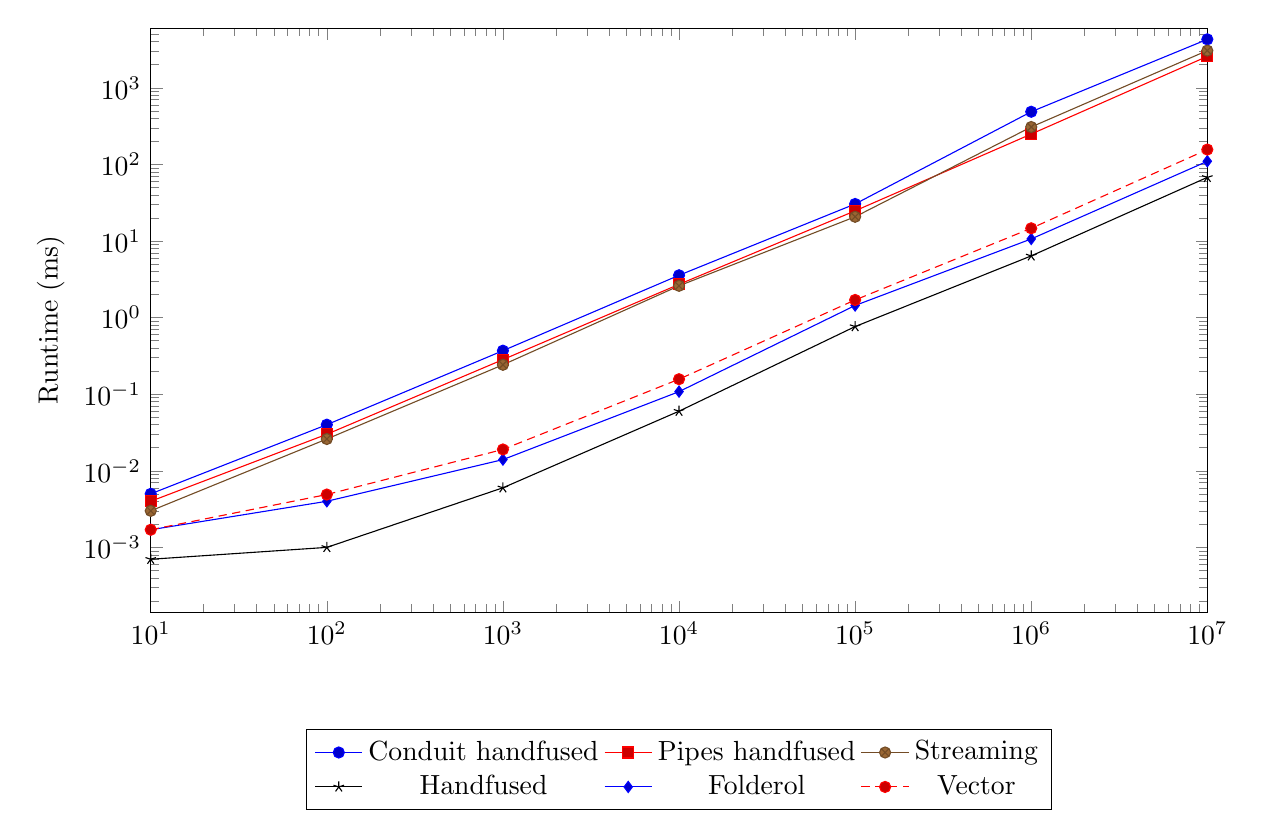
\begin{tikzpicture}
\begin{axis}[
  xtick=data, ylabel=Runtime (ms),
  % All pictures need to specify same upper and lower bounds so they line up together
  ymin=0, ymax=6000,
  xmin=10, xmax=10000000,
  xmode=log, ymode=log,
  width=15cm, height=9.0cm,
  legend style={at={(0.5,-0.2)},anchor=north, legend columns=3},
]

% Conduit two-pass
% \addplot coordinates {(10, 0.015) (100, 0.077) (1000,0.567) (10000,5.14) (100000,47.37) (1000000,512.9) (10000000,5289)  };
\addplot coordinates {(10, 0.005) (100, 0.040) (1000,0.370) (10000,3.57) (100000,30.46) (1000000,487.1) (10000000,4296)  };
\addplot coordinates {(10, 0.004) (100, 0.030) (1000,0.283) (10000,2.72) (100000,24.77) (1000000,249) (10000000,2574)  };
\addplot coordinates {(10, 0.003) (100, 0.026) (1000,0.242) (10000,2.60) (100000,20.72) (1000000,308) (10000000,3065)  };
\addplot coordinates {(10,0.0007) (100,0.001) (1000,0.006) (10000,0.060) (100000,0.764) (1000000,6.393) (10000000,67.71)  };
\addplot coordinates {(10,0.0017) (100,0.004) (1000,0.014) (10000,0.108) (100000,1.44) (1000000,10.64) (10000000,109.9)  };
\addplot coordinates {(10,0.0017) (100,0.0049) (1000,0.019) (10000,0.157) (100000,1.70) (1000000,14.66) (10000000,156.3)  };
% Vector store
% \addplot coordinates {(10,0.0021) (100,0.0059) (1000,0.021) (10000,0.194) (100000,2.37) (1000000,19.18) (10000000,215.3)  };

\legend{Conduit handfused, Pipes handfused, Streaming, Handfused, Folderol, Vector}
\end{axis}

\end{tikzpicture}
\caption{Quickhull runtime; lower is faster.}
\label{fig:bench:quickhull}
\end{figure}

